\documentclass[compress,red]{beamer}
\usepackage[utf8]{inputenc}
\usepackage{ucs}
\usepackage{amsmath}
\usepackage{amsfonts}
\usepackage{amssymb}
\usepackage[russian]{babel}
\usepackage{graphicx}
\usepackage{wrapfig}

\usepackage{tikz}
\usepackage{verbatim}

\usepackage{color}
\usepackage{xcolor}
\usepackage{listings}

\usepackage{caption}

\lstset{
language=ruby,
extendedchars=\true,
inputencoding=utf8x,
commentstyle=\itshape,
stringstyle=\bf,
belowcaptionskip=5pt }


\DeclareCaptionFont{white}{\color{white}}
\DeclareCaptionFormat{listing}{\colorbox{gray}{\parbox{\textwidth}{#1#2#3}}}
\captionsetup[lstlisting]{format=listing,labelfont=white,textfont=white}

\usetikzlibrary{calc,trees,positioning,arrows,chains,shapes.geometric,%
    decorations.pathreplacing,decorations.pathmorphing,shapes,%
    matrix,shapes.symbols}

\tikzset{
>=stealth',
  punktchain/.style={
    rectangle, 
    rounded corners, 
    % fill=black!10,
    draw=black, very thick,
    text width=10em, 
    minimum height=3em, 
    text centered, 
    on chain},
  line/.style={draw, thick, <-},
  element/.style={
    tape,
    top color=white,
    bottom color=blue!50!black!60!,
    minimum width=8em,
    draw=blue!40!black!90, very thick,
    text width=10em, 
    minimum height=1.5em, 
    text centered, 
    on chain},
  every join/.style={->, thick,shorten <=1pt},
  decoration={brace},
  tuborg/.style={decorate},
  tubnode/.style={midway, right=2pt},
}

\mode<presentation>

\usetheme{Warsaw}

\definecolor{Red}{rgb}{1,0,0}
\definecolor{Blue}{rgb}{0,0,1}
\definecolor{Green}{rgb}{0,1,0}
\definecolor{magenta}{rgb}{1,0,.6}
\definecolor{lightblue}{rgb}{0,.5,1}
\definecolor{lightpurple}{rgb}{.6,.4,1}
\definecolor{gold}{rgb}{.6,.5,0}
\definecolor{orange}{rgb}{1,0.4,0}
\definecolor{hotpink}{rgb}{1,0,0.5}
\definecolor{newcolor2}{rgb}{.5,.3,.5}
\definecolor{newcolor}{rgb}{0,.3,1}
\definecolor{newcolor3}{rgb}{1,0,.35}
\definecolor{darkgreen1}{rgb}{0, .35, 0}
\definecolor{darkgreen}{rgb}{0, .6, 0}
\definecolor{darkred}{rgb}{.75,0,0}

\xdefinecolor{olive}{cmyk}{0.64,0,0.95,0.4}
\xdefinecolor{purpleish}{cmyk}{0.75,0.75,0,0}

\useoutertheme[subsection=false]{smoothbars}

\title{Логические задачи}

%\usecolortheme{dolphin}


\begin{document}
%%титульная страница
\maketitle
%% основные моменты

\section{Логика}

\subsection{Парадокс брадобрея}
\begin{frame}[fragile]
  \frametitle{Парадокс брадобрея}
  \begin{itemize}
    \item В некотором городе все мужчины либо бреются сами, либо бреются у единственного в городе брадобрея. В этом же городе есть закон, согласно которому брадобрей бреет только тех людей, кто не бреется сам. Вопрос: бреет ли брадобрей сам себя?
  \end{itemize}
\end{frame}

\subsection{Решение парадокса брадобрея}
\begin{frame}[fragile]
  \frametitle{Решение парадокса брадобрея}
  \begin{enumerate}
    \item Предположение: допустим, существование такого брадобрея возможно. Очевидно, что брить себя сам он не может, так как в этом случае он подпадает под первую категорию (бреющиеся сами). Следовательно, он не бреется. Может ли человек не бриться? Да, если он --- женщина.
    \item В математике 0 --- тоже ответ. Корректный ответ, если дополнить условие задачи замечанием о поле брадобрея: таких городов не существует.
    \item Брадобрей может вообще не бриться. Прецеденты были. Не бреется => нет противоречия.\footnote{На самом деле, если аккуратно поставить все условия, данный парадокс невозможно решить.}
  \end{enumerate}
\end{frame}

\subsection{Парикмахер}
\begin{frame}
  \begin{center}
    \Large{Почему парикмахер в Женеве охотнее подстрижёт двух французов, чем одного немца?}
  \end{center}
\end{frame}

\subsection{Парикмахер ответ}
\begin{frame}
  \begin{center}
    \Huge{Заработает больше}
  \end{center}
\end{frame}

\subsection{Месяцы}
\begin{frame}
  \begin{center}
    \Huge{Сколько месяцев в году имеют 28 дней?}
  \end{center}
\end{frame}

\subsection{Месяцы ответ}
\begin{frame}
  \begin{center}
    \Huge{Все (12)}
  \end{center}
\end{frame}

\subsection{Поезда}
\begin{frame}
  \begin{center}
    \Large{На одном участке двухпутная железная дорога ныряет в туннель и сменяется однопутной. Разминуться внутри туннеля поездам негде. Прошлым летом в туннель с одной стороны на полной скорости влетел поезд. Другой поезд влетел на полной скорости с другой стороны. Никакого столкновения не произошло. Почему?}
  \end{center}
\end{frame}

\subsection{Поезда ответ}
\begin{frame}
  \begin{center}
    \Huge{Они заехали в туннель в разное время}
  \end{center}
\end{frame}

\subsection{Лебедь, рак и щука}
\begin{frame}[fragile]
  \frametitle{Лебедь, рак и щука}
  \centerline{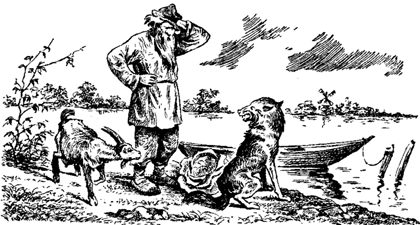
\includegraphics[width=0.8\textwidth]{images/omg.png}}
\end{frame}

\subsection{Лебедь, рак и щука условие}
\begin{frame}[fragile]
  \frametitle{Лебедь, рак и щука}
  \begin{itemize}
    \item Крестьянину нужно перевезти через реку волка, козу и капусту. 
    \item Но лодка такова, что в ней может поместиться только крестьянин, а с ним или только волк, или только коза, или только капуста.
    \item Но если оставить волка с козой, то волк съест козу, а если оставить козу с капустой, то коза съест капусту.
    \item Как перевез свой груз крестьянин?
  \end{itemize}
\end{frame}

\section{Методы исследования}
\subsection{Индукция}
\begin{frame}
  \begin{center}
    \Huge{Индукция}
  \end{center}
  \begin{center}
    \Large{От частного к общему}
  \end{center}
\end{frame}

\subsection{Пример индуктивного рассуждения}
\begin{frame}
  \begin{center}
    \Huge{Корректный пример}
  \end{center}
  \begin{center}
    \Large{Каждую зиму мне было холодно. Следовательно, зимой \textbf{всегда} холодно.}
  \end{center}
\end{frame}

\subsection{Некорректная индукция}
\begin{frame}
  \begin{center}
    \Huge{Некорректный пример}
  \end{center}
  \begin{center}
    \large{
    \begin{itemize}
      \item 3 делится на 3. 
      \item 33 делится на 3. 
      \item 63 делится на 3. 
      \item Следовательно, все числа, оканчивающиеся на 3, делятся на 3.
    \end{itemize}}
  \end{center}
\end{frame}

\subsection{Метод полной индукции}
\begin{frame}[fragile]
  \frametitle{Метод полной индукции}
  \begin{itemize}
    \item Состоит из двух частей:
      \begin{enumerate}
        \item База. Проверяем корректность утверждения на нескольких последовательных примерах.
        \item Переход. Доказываем, что если для всего предыдущего утверждение верно, то он верно и для последующего.
      \end{enumerate}
  \end{itemize}
\end{frame}

\subsection{Пример полной индукции}
\begin{frame}[fragile]
  \frametitle{Пример полной индукции}
  \begin{itemize}
    \item \textbf{Задача.} Докажем, что $1+2+\ldots+n = \cfrac{n\cdot(n+1)}{2}$.
    \item Доказательство:
      \begin{itemize}
        \item База. Проверим при n=2: $1+2 = 3 = \cfrac{2\cdot 3}{2}$.
        \item Переход. Предположим, что формула верна для всех чисел $\leq$ n. Докажем для $n+1$:
          \begin{itemize}
            \item $1+2\ldots +n + (n+1) = \cfrac{n\cdot (n+1)}{2} + (n+1) =$
            \item $ = \cfrac{n\cdot (n+1) + 2\cdot(n+1)}{2} = \cfrac{(n+1)\cdot (n+2)}{2}$, ч.т.д. 
          \end{itemize}
      \end{itemize}
    
  \end{itemize}
\end{frame}

\subsection{Дедукция}
\begin{frame}
  \begin{center}
    \Huge{Дедукция}
  \end{center}
  \begin{center}
    \Large{От общего к частному}
  \end{center}
\end{frame}

\subsection{Примеры дедукции}
\begin{frame}
  \begin{center}
    \Huge{Пример --- силлогизм}
  \end{center}
  \begin{center}
    \Large{
      \begin{itemize}
        \item Все алкоголики долго не живут.
        \item Вася --- алкоголик.
        \item Следовательно, Вася не будет долго жить.
      \end{itemize}
    }
  \end{center}
\end{frame}

\section{Методы решения}

\subsection{Профессия}
\begin{frame}[fragile]
  \centerline{
\includegraphics[width=0.8\textwidth]{images/soccer.jpg}}
\end{frame}

\subsection{Задача 1}
\begin{frame}[fragile]
  \frametitle{Задача 1}
  \begin{itemize}
    \item Четыре футбольных команды: итальянская команда ``Милан'', испанская – ``Реал'', российская – ``Зенит'', английская – ``Челси'' встретились в групповом этапе лиги чемпионов по футболу. Их тренировали тренеры из этих же четырех стран: итальянец Антонио, испанец Родриго, русский Николай, англичанин Марк. Известно, что национальность у всех четырех тренеров не совпадала с национальностью команд. Требуется определить тренера каждой команды, если известно: 
    \begin{enumerate}
      \item Зенит не тренируется у Марка и Антонио. 
      \item Милан обещал никогда не брать Марка главным тренером.
    \end{enumerate}
  \end{itemize}
\end{frame}

\subsection{Графы 1}
\begin{frame}[fragile]
  \frametitle{Решение с помощью графов}
  \centerline{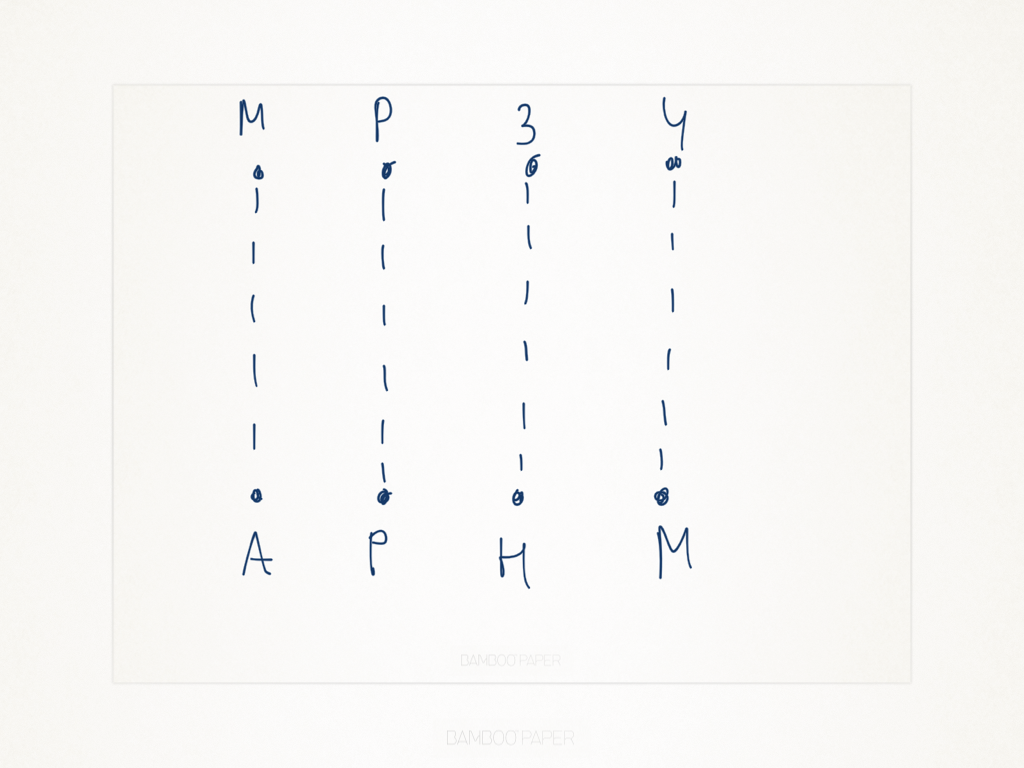
\includegraphics[width=0.6\textwidth]{images/graph-01.png}}
  \begin{itemize}
    \item Сверху --- команды, снизу --- тренера.
    \item Пунктир --- кто \textbf{не может} тренировать команду.
  \end{itemize}
\end{frame}

\subsection{Графы 2}
\begin{frame}[fragile]
  \frametitle{Решение с помощью графов}
  \centerline{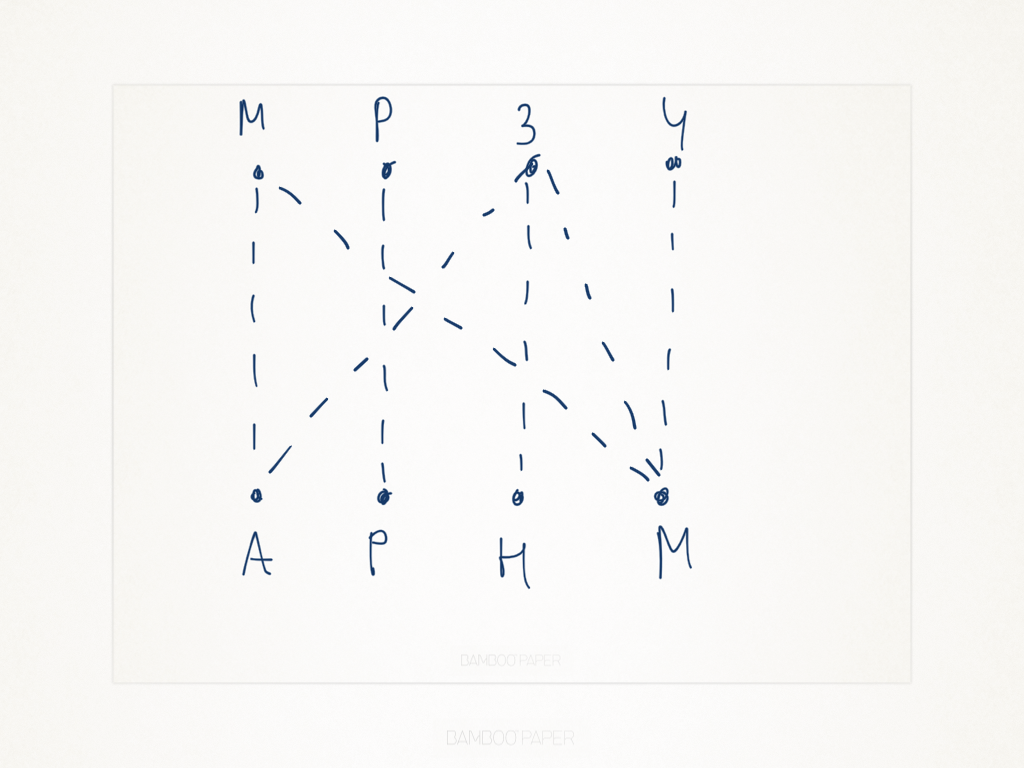
\includegraphics[width=0.6\textwidth]{images/graph-02.png}}
  \begin{itemize}
    \item Добавим оба условия: (Зенит не тренируется у Марка и Антонио) и (Милан обещал никогда не брать Марка главным тренером).
  \end{itemize}
\end{frame}

\subsection{Графы 3}
\begin{frame}[fragile]
  \frametitle{Решение с помощью графов}
  \centerline{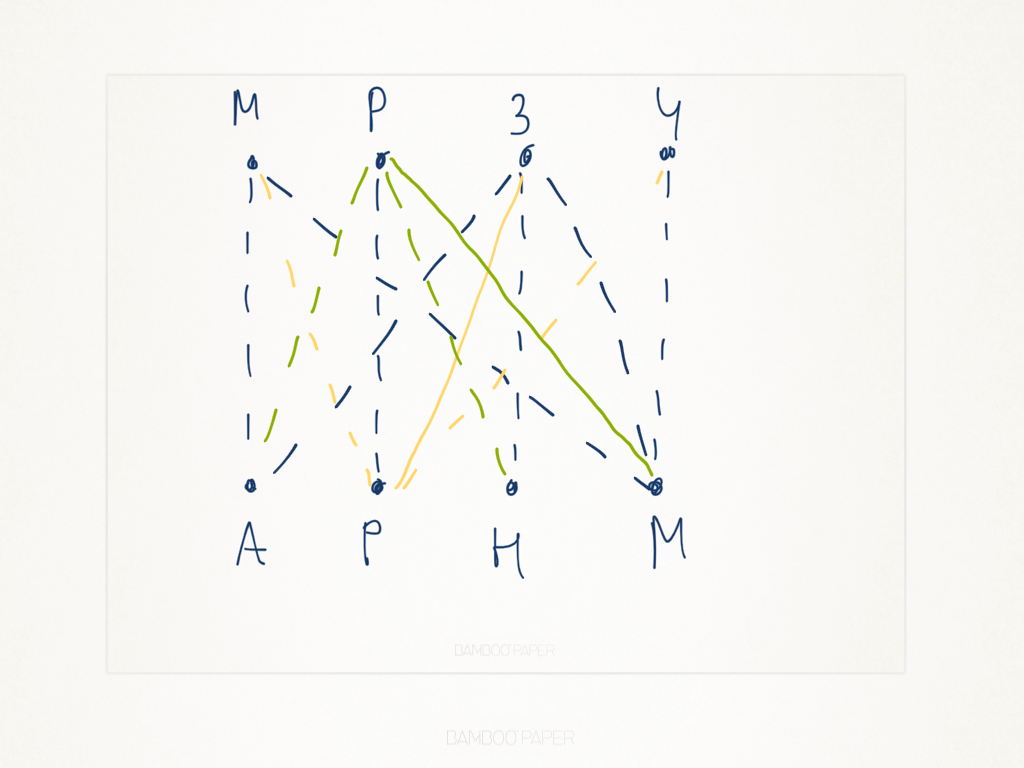
\includegraphics[width=0.6\textwidth]{images/graph-03.png}}
  \begin{itemize}
    \item Следовательно, Зенит тренирует Родриго.
    \item Марк тренирует Реал.
    \item Милан --- Николай, Челси --- Антонио.
  \end{itemize}
\end{frame}

\subsection{Таблицы 1}
\begin{frame}[fragile]
  \frametitle{Решение с помощью таблиц}
  
  \center
  {
  \begin{tabular}{|c|c|c|c|c|}
    \hline
    Имя & Милан & Реал  & Зенит & Челси \\
    \hline
    Антонио & --- &   & & \\
    \hline
    Родриго &  & ---  &  & \\
    \hline
    Николай &  &   & ---  & \\ 
    \hline
    Марк &  &   &  & --- \\
    \hline
  \end{tabular}
  }
  \begin{itemize}
    \item Минусы --- кто не может тренировать, плюсы --- кто тренирует.
  \end{itemize}
\end{frame}

\subsection{Таблицы 2}
\begin{frame}[fragile]
  \frametitle{Решение с помощью таблиц}
  
  \center
  {
  \begin{tabular}{|c|c|c|c|c|}
    \hline
    Имя & Милан & Реал  & Зенит & Челси \\
    \hline
    Антонио & --- &   & --- & \\
    \hline
    Родриго &  & ---  &  & \\
    \hline
    Николай &  &   & ---  & \\ 
    \hline
    Марк & --- &   & --- & --- \\
    \hline
  \end{tabular}
  }
  \begin{itemize}
    \item Вносим условия задачи в таблицу.
  \end{itemize}
\end{frame}

\subsection{Таблицы 3}
\begin{frame}[fragile]
  \frametitle{Решение с помощью таблиц}
  
  \center
  {
  \begin{tabular}{|c|c|c|c|c|}
    \hline
    Имя & Милан & Реал  & Зенит & Челси \\
    \hline
    Антонио & --- &   & --- & \\
    \hline
    Родриго & ---  & ---  & +  & --- \\
    \hline
    Николай &  &   & ---  & \\ 
    \hline
    Марк & --- &   & --- & --- \\
    \hline
  \end{tabular}
  }
  \begin{itemize}
    \item Зенит может тренировать только Родриго.
    \item Если Родриго тренирует Зенит, больше никого тренировать он не может.
  \end{itemize}
\end{frame}

\subsection{Таблицы 4}
\begin{frame}[fragile]
  \frametitle{Решение с помощью таблиц}
  
  \center
  {
  \begin{tabular}{|c|c|c|c|c|}
    \hline
    Имя & Милан & Реал  & Зенит & Челси \\
    \hline
    Антонио & --- &   & --- & \\
    \hline
    Родриго & ---  & ---  & +  & --- \\
    \hline
    Николай & + & ---  & ---  & --- \\ 
    \hline
    Марк & --- &   & --- & --- \\
    \hline
  \end{tabular}
  }
  \begin{itemize}
    \item Милан может тренировать только Николай, так как никто больше не может.
    \item Раз Милан тренирует Николай, другие команды он тренировать не может.
  \end{itemize}
\end{frame}

\subsection{Таблицы 4}
\begin{frame}[fragile]
  \frametitle{Решение с помощью таблиц}
  
  \center
  {
  \begin{tabular}{|c|c|c|c|c|}
    \hline
    Имя & Милан & Реал  & Зенит & Челси \\
    \hline
    Антонио & --- & ---   & --- & + \\
    \hline
    Родриго & ---  & ---  & +  & --- \\
    \hline
    Николай & + & ---  & ---  & --- \\ 
    \hline
    Марк & --- & + & --- & --- \\
    \hline
  \end{tabular}
  }
  \begin{itemize}
    \item Челси может тренировать только Антонио.
    \item По методу исключения Реал тренирует Марк.
  \end{itemize}
\end{frame}

\section{Задачи}
\subsection{Четыре поросёнка}
\begin{frame}[fragile]
  \frametitle{Задача}
  \begin{itemize}
    \item Атос, Портос, Арамис и Д’Артаньян --- четыре талантливых молодых мушкетёра. Один из них лучше всех сражается на шпагах, другой не имеет равных в рукопашном бою, третий лучше всех танцует на балах, четвертый без промаха стреляет с пистолетов. О них известно следующее: 
    \begin{enumerate}
      \item Атос и Арамис наблюдали на балу за их другом --- прекрасным танцором. 
      \item Портос и лучший стрелок вчера с восхищением следили за боем рукопашника.
      \item Стрелок хочет пригласить в гости Атоса.
      \item Портос был очень большой комплекции, поэтому танцы были не его стихией.
    \end{enumerate}
    \item Кто чем занимается?
  \end{itemize}
\end{frame}

\subsection{Три хряка}
\begin{frame}[fragile]
  \frametitle{Задача}
  \begin{itemize}
    \item Жили-были на свете три поросенка, три брата: Ниф-Ниф, Наф-Наф, Нуф-Нуф. Построили они три домика: соломенный, деревянный и кирпичный. Все три брата выращивали возле своих домиков цветы: розы, ромашки и тюльпаны. Известно, что Ниф-Ниф живет не в соломенном домике, а Наф-Наф – не в деревянном; возле соломенного домика растут не розы, а тот, у кого деревянный домик, выращивает ромашки. У Наф-Наф аллергия на тюльпаны, поэтому он не выращивает их. Узнайте, кто в каком домике живет и какие цветы выращивает. 
  \end{itemize}
\end{frame}

\subsection{Гарри Поттер и логика}
\begin{frame}[fragile]
  \frametitle{Гарри Поттер}
  \begin{itemize}
    \item Однажды на лестнице Гарри Поттер нашел странный свиток. В нем было записано сто утверждений:
    \begin{enumerate}
      \item В этом свитке ровно одно неверное утверждение.
      \item В этом свитке ровно два неверных утверждения.
      \item В этом свитке ровно три неверных утверждения.
      \item ...
      \item В этом свитке ровно сто неверных утверждений.
    \end{enumerate}
    \item Есть ли среди этих утверждений верные, и если да, то какие?
  \end{itemize}
\end{frame}

\subsection{Задача Эйнштейна}
\begin{frame}[fragile]
  \frametitle{Задача Эйнштейна}
  \begin{itemize}
    \item На одной улице подряд стоят пять домов, каждый — своего цвета. В каждом живёт человек, все пять — разных национальностей. Каждый человек любит свою марку сигарет, напиток и домашнее животное. Также:
    \begin{enumerate}
      \scriptsize
      {
      \item Норвежец живёт в первом доме.
      \item Англичанин живёт в красном доме.
      \item Зелёный дом находится слева от белого, рядом с ним.
      \item Датчанин пьёт чай.
      \item Тот, кто курит Marlboro, живёт рядом с тем, кто выращивает кошек.
      \item Тот, кто живёт в жёлтом доме, курит Dunhill.
      \item Немец курит Rothmans.
      \item Тот, кто живёт в центре, пьёт молоко.
      \item Сосед того, кто курит Marlboro, пьёт воду.
      \item Тот, кто курит Pall Mall, выращивает птиц.
      \item Швед выращивает собак.
      \item Норвежец живёт рядом с синим домом.
      \item Тот, кто выращивает лошадей, живёт в синем доме.
      \item Тот, кто курит Winfield, пьет пиво.
      \item В зелёном доме пьют кофе.
      }
    \end{enumerate}    
    \item Кто разводит рыбок?
  \end{itemize}
\end{frame}

\end{document}